\scanpage{71}
\mspage{\deleted{\unsure{69|79}}\unsure{70|79}}

Il revient au $=$ de dire que $F$ et $F'$ ont $=$ cosupport, ou encore, même support.

\unsure{Donnons nous} un support.

% Figure L1: the two broken vertical groups in the left margin; no linguistic function assigned.
\margin{\figure{\begin{tikzpicture}[x=0.009cm,y=0.009cm,line cap=round]
\fill (0,0) ellipse (1.7 and 2.6);
\draw[line width=0.9pt] (-0.5,-5) -- (0.6,-10) -- (-0.5,-15);
\draw[line width=0.9pt] (0,-20) -- (1,-25) -- (-0.7,-31);
\fill (8,-35) ellipse (1.4 and 1.8);
\fill (195,31) circle (1.5);
\draw[line width=0.8pt] (194,27) -- (196,23) -- (194,21);
\fill (196,17) circle (1.4);
\fill (196,11) circle (1.3);
\fill (194,-2) circle (1.6);
\end{tikzpicture}}}
Une autre façon de dire que $F,G\ \text{disj.}\Longrightarrow F',G\ \text{disj}$, est ainsi :

\uline{Corollaire}
% Figure L2: raised insertion and its curved oblique arm; the arm crosses the older de.
\figure{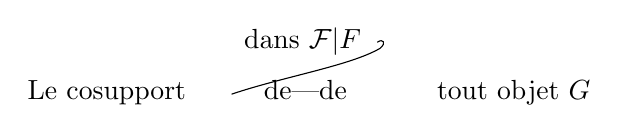
\begin{tikzpicture}[x=1cm,y=1cm,line cap=round]
\node[anchor=base west,inner sep=0pt] at (0,0) {Le cosupport};
\node[anchor=base west,inner sep=0pt] at (3.0,0) {\unsure{de|\deleted{de}}};
\node[anchor=base west,inner sep=0pt] at (5.2,0) {tout objet $G$};
\node[anchor=base west,inner sep=0pt] at (2.75,0.65) {\inserted{dans $\unsure{\mathcal F|F}$}};
\draw (2.60,0.07) .. controls (3.25,0.29) and (4.10,0.43) .. (4.48,0.65)
 .. controls (4.57,0.72) and (4.52,0.78) .. (4.45,0.73);
\end{tikzpicture}}
de $\mathcal F$ est fermé, non seult pour $\leq$, mais aussi pour $\preceq$ -- c'est donc ce qu'on appelle une \uline{sous}-\unsure{contrée|contrie}.

Donc \unsure{itou} pour toute partie $\Phi\subset\mathcal F$.

En d'autres termes, \deleted{toute} partie de $\mathcal F$ qui est un $\mathcal F$-support (ou ``$\mathcal F$-saturée, sous-entendu :
% Figure L3: crowded punctuation at the right edge after the order sign; identities remain open.
\figure{
\begin{tikzpicture}[x=1cm,y=1cm,line cap=round]
\node[anchor=base west,inner sep=0pt] at (0,0) {en termes de $\leq$};
\draw[line width=0.6pt] (3.27,-0.04) .. controls (3.30,-0.14) and (3.22,-0.23) .. (3.16,-0.28);
\draw[line width=0.6pt] (3.42,0.43) .. controls (3.68,0.10) and (3.66,-0.15) .. (3.45,-0.32);
\draw[line width=0.6pt] (3.56,0.28) .. controls (3.70,0.24) and (3.89,0.20) .. (3.71,0.08)
 -- (3.63,0.01) .. controls (3.77,-0.03) and (3.83,-0.08) .. (3.94,-0.10);
\end{tikzpicture}}
cf page $67$) est \unsure{automatiquemt|automatiquement} \deleted{\unsure{f}}une sous-contrée.

% Figure L4: long separator with a downward notch and a rounded descending right end, in scan orientation.
\figure{\begin{tikzpicture}[x=0.006cm,y=0.006cm,line cap=round]
\draw (118,0) .. controls (230,15) and (355,37) .. (441,35)
 .. controls (463,33) and (463,0) .. (492,0)
 .. controls (535,3) and (558,17) .. (592,20)
 .. controls (890,31) and (1325,69) .. (1606,70)
 .. controls (1642,70) and (1641,38) .. (1648,-18)
 .. controls (1652,-92) and (1650,-160) .. (1680,-220);
\end{tikzpicture}}
% Cancelled draft is written upside down on the sheet; the long oblique strokes cancel the entire text block.
% Its text is given below in its own reading order. The folio belongs to that cancelled draft.
\mspage{\deleted{5\deleted{\unsure{4|3}}5}}

\deleted{un ensemble, et $\deleted{\unsure{\mathcal F|F}}\Phi$ un ens de parties de $M$, satisfaisant la condition précédente \unsure{(au --)|(ou --)|(en --)}.}

\deleted{Alors $\Phi$, muni de la relation d'inclusion, satisfait $C\,1$, et ses objets irréductibles sont les $A_x$ $(x\in M)$, l'application $x\mathrel{\vdash\joinrel\dashv} A_x$ étant une bijection de $M$ sur l'ens}
% Figure L5: penultimate line of the inverted cancelled draft, shown upright for reading.
% The point above the second internal deletion and two low points beneath irreductibles are retained.
\figure{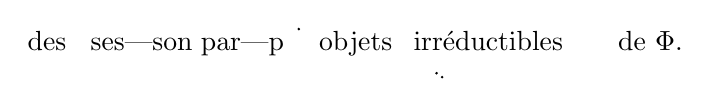
\begin{tikzpicture}[x=1cm,y=1cm,line cap=round]
\node[anchor=base west,inner sep=0pt] at (0,0) {\deleted{des}};
\node[anchor=base west,inner sep=0pt] at (0.8,0) {\deleted{\deleted{\unsure{ses|son}}}};
\node[anchor=base west,inner sep=0pt] at (2.2,0) {\deleted{\deleted{\unsure{par|p}}}};
\node[anchor=base west,inner sep=0pt] at (3.7,0) {\deleted{objets}};
\node[anchor=base west,inner sep=0pt] at (4.9,0) {\deleted{irréductibles}};
\node[anchor=base west,inner sep=0pt] at (7.5,0) {\deleted{de $\Phi$.}};
\fill (3.45,0.27) circle (0.018);
\fill (5.20,-0.29) circle (0.018);
\fill (5.27,-0.34) circle (0.018);
\end{tikzpicture}}

\deleted{Dém $A_x$ est irréductible, car si $A_x=\bigcup_{i\in I} A_i$}
